\section{The Leap Motion Controller}
The latest technological breakthrough in gesture-sensing devices has come in the form of a Leap Motion Controller (Leap Motion, San Francisco, CA, United States). The controller, approximately the size of a box of matches, allows for the precise and fluid tracking of multiple hands, fingers, and small objects in free space with sub-millimeter accuracy~\citep{Guna2014}.

\subsection{Physical Properties}
The Leap Motion Controller (see fig. \ref{fig:leapmotion} and \ref{fig:leapmotion2}) contains two stereoscopic cameras and three infrared LEDs, which periodically emit a light pulse with a wavelength of 850 nanometer, and thus outside the visible light spectrum. During the light pulses, which light up about eight cubic feet in front of the controller, grayscale stereo images are captured by the cameras and sent to the Leap Motion tracking software~\citep{LeapMotion2016}. In the software, the images are analysed to reconstruct a 3D representation of what the device sees, compensating for static background objects and ambient environmental lighting. 

\begin{figure}%[h!] %[H]
	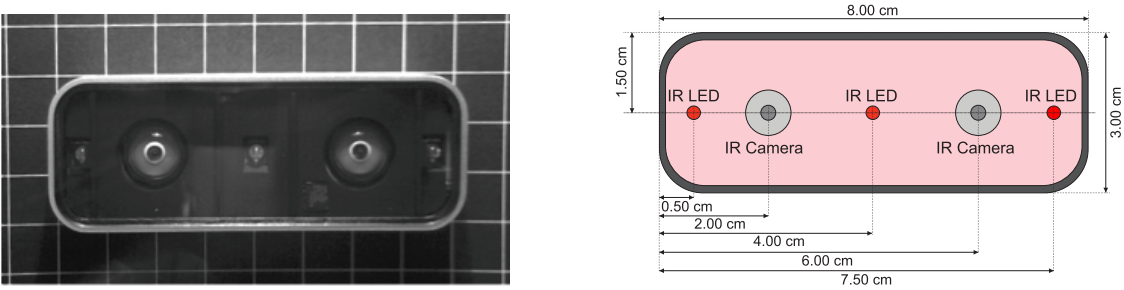
\includegraphics[width=\linewidth]{pictures/LMC_measures.png}
	\caption{Visualization of a Leap Motion Controller, with Infrared Imaging (left) and a Schematic View (right)~\citep{Weichert2013}.}
	\label{fig:leapmotion2}
\end{figure} 

\subsection{The Leap API}
The controller itself can be accessed and programmed through Application Programming Interfaces (APIs), with support for a variety of programming languages, including C++, C\#, Objective-C, Java, JavaScript and Python. Although the API is programmed almost exclusively in C, access through a variety of other languages is achieved by virtue of various "wrapper libraries", which exposes and translates functions from their respective languages into the corresponding C function[cite].

The Leap Motion SDK also features integration with commercial game engines such as Unity and the Unreal Engine~\citep{Guna2014}. One example of what the Leap Motion API enables is acquisition of the recognized object's position through Cartesian and spherical coordinate systems, which are used to describe positions in the controller's sensory space~\citep{Guna2014}.  

Technically, very few details are publicly known about the precise nature of the algorithms used due to patent and trade secret restrictions.

\subsection{Important Leap components}
Hands, fingers, palm, directions, frames, interaction box etc. See \\
https://developer.leapmotion.com/documentation/csharp/devguide/Leap\_Overview.html\#motion-tracking-data \\
https://developer.leapmotion.com/documentation/csharp/devguide/Leap\_Coordinate\_Mapping.html\#map3d \\
https://developer.leapmotion.com/documentation/csharp/devguide/Leap\_Hand.html \\


\subsection{Detectors - The building blocks of gesture recognition}
The detector scripts. How they can be combined. Logic gates. 
See https://developer.leapmotion.com/documentation/unity/unity/Unity\_DetectionUtilities.html

\subsection{Integration with the Unity editor}
How the pieced fit together. How the stuff is organized (e.g the modules).
See https://developer.leapmotion.com/documentation/unity/index.html